Even though the design requirements are included in the computation of the different configurations, it is necessary to evaluate how does the constellation perform when deployed. With this purpose, another MATLAB routine was developed. 

\paragraph{Time factor\\}
It is important to remark that the design methods used so far did not consider coverage in a certain period of time, but the coverage at a given instant. This section summarizes a method to compute this variation.

\paragraph{Quality Time\\}
Another factor that was not considered in the design process was the pass times of the satellites. If a pass is too short the contact with the satellite cannot be produced. 

\subsection{Performance Evaluation}
In order to determine if the performance of the Constellation is good enough and to compare different constellations, we define the following parameters that are to be used in the weighted ordered average decision\ref{OWA-Constellation}.\\
\newline
Simulation parameters important to clarify:
\begin{itemize}
\item Simulation time: 25h. This time is enough to observe the motion of the whole constellation on Earth considering its rotation and the rotation of the plains due to the Earth's oblateness.
\item Minimum contact time: 3 minutes. Time enough to download data, tracking and Telecommanding the satellite.
\item Time precision: 10 seconds. It is empirically observed to be precise enough.
\end{itemize}

The computed parameters:\label{PerfAnal}
\begin{itemize}
\item Fraction of time with flybys on the GS: Ratio between the time in which there is any satellite in the field of view of the Ground Station and the total simulation time. (Referred in table \ref{OWA-Constellation} as \% Coverage)
\item Mean number of links with the satellite
\item Fraction of time with flybys longer than 3 minutes: In this case the ratio is with the time in which there is a satellite doing a useful pass, since a full contact can be done. (Referred in table \ref{OWA-Constellation} as \%Quality Time) 
\item Mean pass time: This parameter is used to guarantee a minimum of quality and to compare different configurations. (Referred in table \ref{OWA-Constellation} as Average Pass Time)
\item Number of gaps: Gaps are in this chapter defined as periods of time without a pass that is lasting/will last more than 3 minutes. (Referred in table \ref{OWA-Constellation} as Num Gaps)
\item Maximum gap time: At high latitudes all the Walker-Delta configurations show a characteristic gap that can last even for hours, which is not admissible. This parameter will tell us if we exceed a maximum defined as 3 minutes for this study. (Referred in table \ref{OWA-Constellation} as Max Gap Time)
\item Mean gap time: As it is obvious, a minimum or a 0 is desired. 
\end{itemize}

You can find below an example of the analysis, for a constellation in a Semi Walker-Delta configuration.

\begin{table}[H]
\centering
\begin{tabular}{|l|c|}
\hline
Constellation & Full WD \\ \hline
Number of Planes     & $ p=8 $   \\ \hline
Satellites per plane   & $ spp=18 $ \\ \hline
Inclination  	 & $ i=75º $   \\ \hline
GS Latitude   & $ \lambda=80º$   \\ \hline
GS Longitude & $ \phi=0º $ \\ \hline
\end{tabular}
\caption{Constellation parameters for the Example Constellation}
\end{table}

\begin{figure}[H]
\begin{center}
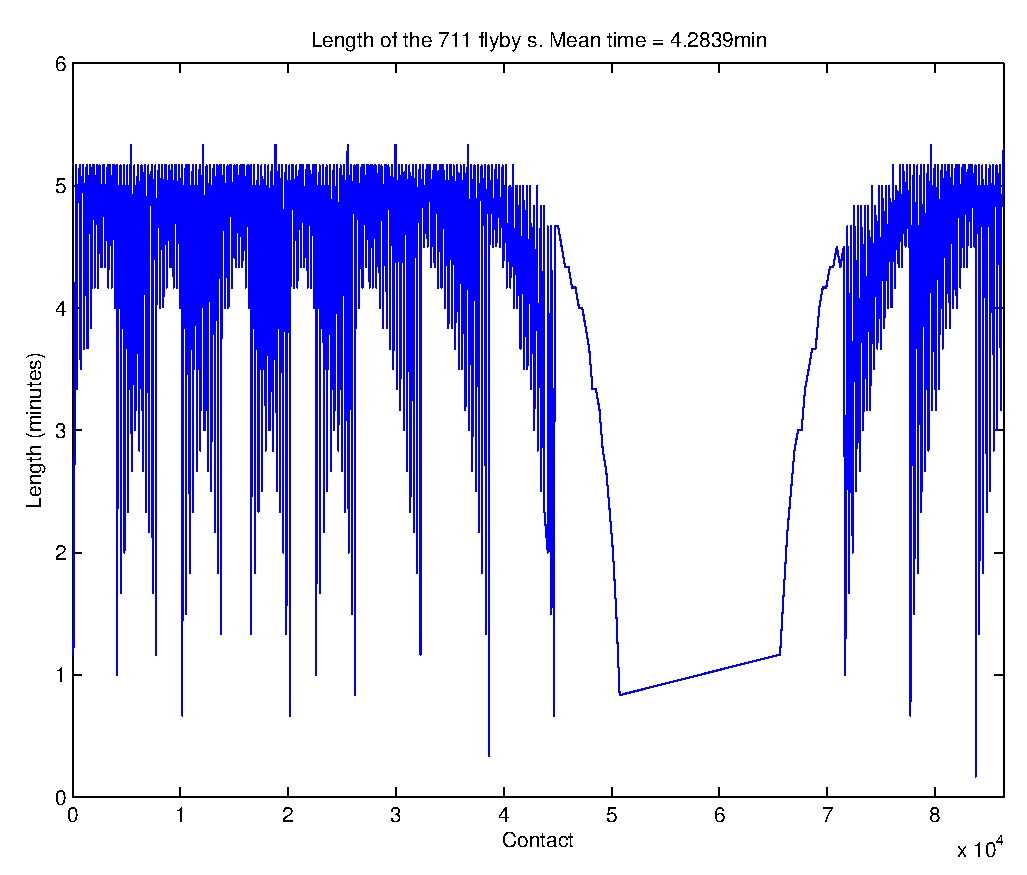
\includegraphics[scale=0.8]{LengthPass}
\caption{Length of the passes on the example GS.}
\end{center}
\end{figure}

\begin{table}[H]
\centering

\begin{tabular}{|l|c|}
\hline
Pass Time Ratio & $77.53\% $ \\ \hline
Quality Time Ratio     & $ 75.77\% $   \\ \hline
Mean Pass Time   & $ 4.28 min $ \\ \hline
Number of gaps  	 & $37$   \\ \hline
Maximum Gap Time   & $ 314.33 min $   \\ \hline
\end{tabular}
\caption{Performance Parameters for the Example Constellation}
\end{table}

Given the high latitude of the Ground Station plus the Semi Walker-Delta Configuration there is an enormous gap. In addition, between planes some gaps are also observed.